\chapter{Исследовательская часть}

В данном разделе будут приведены примеры работы программы, и будет проведен сравнительный анализ реализованных алгоритмов умножения матриц по затраченному процессорному времени.

\section{Технические характеристики}

Технические характеристики устройства, на котором выполнялось исследование представлены ниже.

\begin{itemize}
	\item операционная система: Manjaro Linux \cite{manjaro};
	\item память : 7,6 GiB;
	\item процессор: 8 × Intel® Core™ i5-10210U CPU @ 1.60GHz \cite{intel}.
\end{itemize}

\clearpage

\section{Демонстрация работы программы}

На рисунке \ref{img:example} приведен пример работы программы.

\begin{figure}[H]
	\begin{center}
		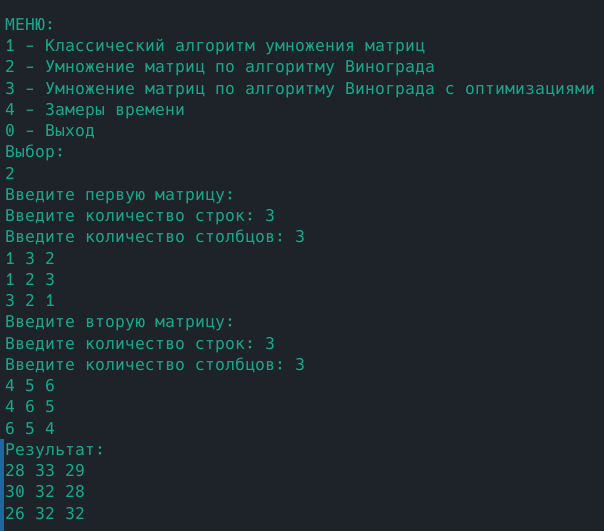
\includegraphics[scale=0.7]{img/example.png}
	\end{center}
	\captionsetup{justification=centering}
	\caption{Пример работы программы}
	\label{img:example}
\end{figure}

\section{Временные характеристики}

Функция process\_time\_ns из библиотеки time языка программирования Python возвращает  процессорное время в наносекундах.

Замеры проводились для матриц размерами от 10х10 до 101х101, заполненных случайными элементами.

На рисунке \ref{img:time} приведены графические результаты сравнения временных характеристик.

\begin{figure}[H]
	\begin{center}
		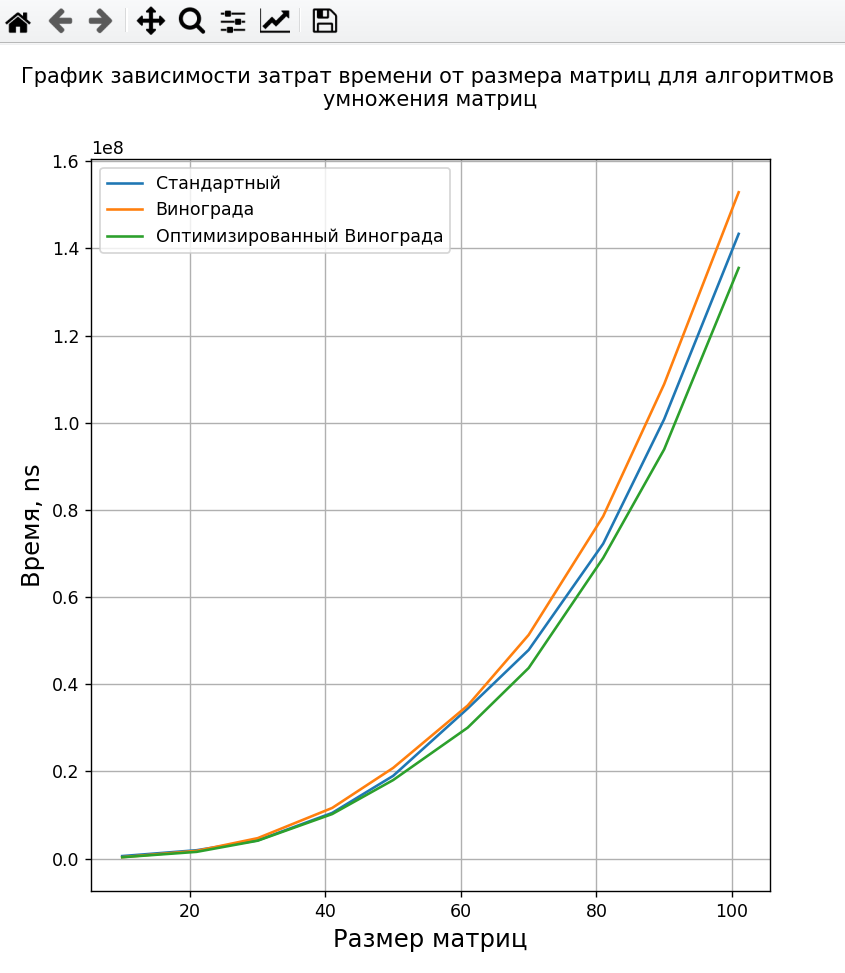
\includegraphics[scale=0.7]{img/time.png}
	\end{center}
	\captionsetup{justification=centering}
	\caption{Сравнение по времени алгоритмов умножения матриц}
	\label{img:time}
\end{figure}

\section{Вывод}
Приведенные характеристики времени показывают нам, что наименее затратным по времени является оптимизированный алгоритм Винограда.